\begin{dang}{Các bài toán thể tích thực tế}
\end{dang}
\subsubsection{Ví dụ minh hoạ}
\begin{vd}[TH]%[1K7KQ-4]
	Từ một tấm bìa hình vuông, người ta cắt ở bốn góc của tấm bìa đó bốn hình vuông bằng nhau, mỗi hình vuông có cạnh bằng $6 \mathrm{~cm}$, rồi gập tấm bìa lại để được một chiếc hộp không nắp có dạng hình hộp chữ nhật.
	\begin{center}
		\begin{tikzpicture}[scale=0.7,x=1cm,y=1cm,line join = round, line cap = round]
			\coordinate[label=left:$$] (D) at (0,0);
			\coordinate [label=left:$$] (A) at (0,6);
			\coordinate [label=right:$$] (B) at (6,6);
			\coordinate [label=right :$$] (C) at (6,0);
			\coordinate [label=right :$$] (E) at (1,0);
			\coordinate [label=right :$$] (F) at (5,0);
			\coordinate [label=right :$$] (G) at (1,6);
			\coordinate [label=right :$$] (H) at (5,6);
			\coordinate [label=right :$$] (I) at (0,5);
			\coordinate [label=right :$$] (J) at (0,1);
			\coordinate [label=right :$$] (M) at (6,1);
			\coordinate [label=right :$$] (N) at (6,5);
			\draw(A)--(B)--(C)--(D)--(A);
			\draw[dashed] (G)--(E)(H)--(F)(I)--(N)(J)--(M);
		\end{tikzpicture}\qquad
		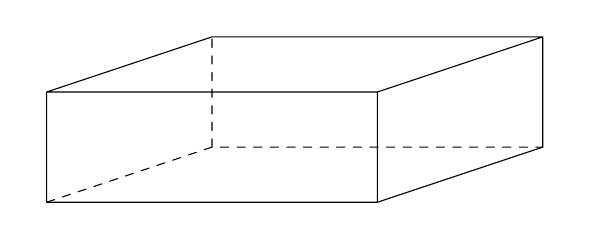
\begin{tikzpicture}[scale=0.7,x=1cm,y=1cm,line join = round, line cap = round]
			\coordinate[label=left:$$] (D) at (0,0);
			\coordinate [label=left:$$] (A) at (3,1);
			\coordinate [label=right:$$] (B) at (6,0);
			\coordinate [label=right :$$] (C) at (9,1);
			\coordinate [label=right :$$] (E) at (0,2);
			\coordinate [label=right :$$] (F) at (6,2);
			\coordinate [label=right :$$] (G) at (3,3);
			\coordinate [label=right :$$] (H) at (9,3);
			\draw(D)--(E)--(G)--(H)--(F)--(E)(D)--(B)--(C)(F)--(B)(C)--(H);
			\draw[dashed] (D)--(A)--(C)(A)--(G);
		\end{tikzpicture}
	\end{center} Tính cạnh của tấm bìa ban đầu, biết rằng thể tích của chiếc hộp bằng $600 \mathrm{~cm}^3$.
	\dapso{22 cm.}
	\loigiai{
		Giả sử tấm bìa ban đầu có cạnh $x~(\mathrm{cm})~(x>12)$. Khi đó đáy của chiếc hộp là hình vuông cạnh $x-12(\mathrm{~cm})$ nên diện tích của đáy chiếc hộp là $(x-12)^2~\left(\mathrm{cm}^2\right)$.\\
		Mà chiều cao của chiếc hộp là $6 \mathrm{cm}$, suy ra thể tích của chiếc hộp bằng $(x-12)^2 \cdot 6~\left(\mathrm{cm}^3\right)$.\\
		Theo đề bài, thể tích của chiếc hộp bằng $600~ \mathrm{cm}^3$ nên
		$$
		(x-12)^2 \cdot 6=600 \Leftrightarrow(x-12)^2=100 .
		$$
		Với $x>12$ ta có: $x-12=10 \Leftrightarrow x=22~(\mathrm{cm})$.\\
		Vậy độ dài cạnh của tấm bìa ban đầu là 22 cm.}
\end{vd}
\begin{vd}[TH]%[1K7KQ-4]
	Từ một tấm tôn hình vuông có cạnh $8 \mathrm{dm}$, bác Hùng cắt bỏ bốn phần như nhau ở bốn góc, sau đó bác hàn các mép lại để được một chiếc thùng (không có nắp)
	\begin{center}
		\begin{tikzpicture}[scale=0.7,x=1cm,y=1cm,line join = round, line cap = round]
			\coordinate[label=left:$$] (D) at (0,0);
			\coordinate [label=left:$$] (A) at (0,6);
			\coordinate [label=right:$$] (B) at (6,6);
			\coordinate [label=right :$$] (C) at (6,0);
			\coordinate [label=right :$$] (E) at (1,0);
			\coordinate [label=right :$$] (F) at (5,0);
			\coordinate [label=right :$$] (G) at (1,6);
			\coordinate [label=right :$$] (H) at (5,6);
			\coordinate [label=right :$$] (I) at (0,5);
			\coordinate [label=right :$$] (J) at (0,1);
			\coordinate [label=right :$$] (M) at (6,1);
			\coordinate [label=right :$$] (N) at (6,5);
			\coordinate [label=right :$$] (P) at (1,1);
			\coordinate [label=right :$$] (Q) at (5,1);
			\coordinate [label=right :$$] (R) at (1,5);
			\coordinate [label=right :$$] (S) at (5,5);
			\draw (R)--(I)--(J)--(P)--(E)--(F)--(Q)--(M)--(N)--(S)--(H)--(G)--(R)--(I);
			\draw[dashed] (R)--(S)--(Q)--(P)--(R);
		\end{tikzpicture}\qquad
		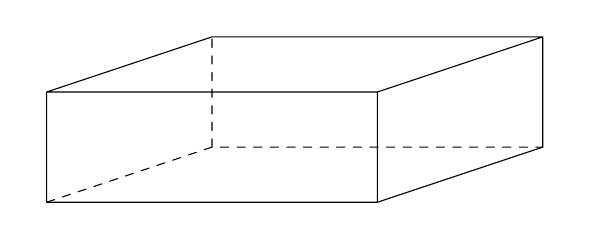
\begin{tikzpicture}[scale=0.7,x=1cm,y=1cm,line join = round, line cap = round]
			\coordinate[label=left:$$] (D) at (0,0);
			\coordinate [label=left:$$] (A) at (3,1);
			\coordinate [label=right:$$] (B) at (6,0);
			\coordinate [label=right :$$] (C) at (9,1);
			\coordinate [label=right :$$] (E) at (0,2);
			\coordinate [label=right :$$] (F) at (6,2);
			\coordinate [label=right :$$] (G) at (3,3);
			\coordinate [label=right :$$] (H) at (9,3);
			\draw(D)--(E)--(G)--(H)--(F)--(E)(D)--(B)--(C)(F)--(B)(C)--(H);
			\draw[dashed] (D)--(A)--(C)(A)--(G);
		\end{tikzpicture}
	\end{center}
	a) Giải thích vì sao chiếc thùng có dạng hình chóp cụt.\\
	b) Tính cạnh bên của thùng.\\
	c) Hỏi thùng có thể chứa được nhiều nhất bao nhiêu lít nước?\\
	\dapso{b) 2dm.	c) 42 lít. }
	\loigiai{
		a) $A B \parallel A' B' \Rightarrow A B \parallel\left(A' B' C' D'\right), A D \parallel A' D' \Rightarrow A D \parallel\left(A' B' C' D'\right)$.\\
		Do đó $(A B C D) \parallel\left(A' B' C' D\right)$.\\
		b) Cạnh bên của hình chóp cụt bằng $\sqrt{\dfrac{9}{4}+\dfrac{25}{4}}=\dfrac{\sqrt{34}}{2}$ (dm).\\
		c) Xét mặt chứa đường chéo của hình vuông, nó là hình thang cân có chiều cao bằng chiều cao của hình chóp cụt và tính ra được $h=\sqrt{\dfrac{34}{4}-\dfrac{18}{4}}=2~(\mathrm{dm})$.
		Thể tích cần tìm là $V=42$ lít.}
\end{vd}
\subsubsection{Bài tập vận dụng}
\begin{bt}[TH]%[1K7KQ-4] 
	\immini{Một sọt đựng đồ có dạng hình chóp cụt đều.
		Đáy và miệng sọt là các hình vuông tương ứng có cạnh bằng $60 \mathrm{~cm}, 30 \mathrm{~cm}$, cạnh bên của sọt dài $50 \mathrm{~cm}$. Tính thể tích của sọt.\\
		\dapso{$48000$ $cm^3$.}}{
		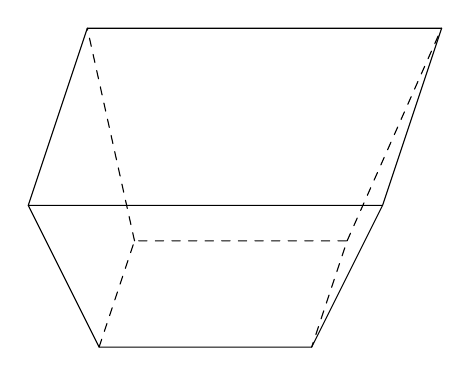
\begin{tikzpicture}[scale=1, font=\footnotesize, line join=round, line cap=round, >=stealth]
			\def\k{0.45}
			\path  
			(1*\k,3*\k) coordinate (A) 
			(7*\k,3*\k) coordinate (B)
			(6*\k,0) coordinate (C)
			(0,0) coordinate (D)
			(-1/3*\k,9*\k) coordinate (A')
			(9*\k+2*\k/3,9*\k) coordinate (B')
			(8*\k,4*\k) coordinate (C')
			(-2*\k,4*\k) coordinate (D')
			; 
			\draw (C)--(D)--(D')--(C')--cycle (C')--(B')--(A')--(D');
			\draw[dashed] (D)--(A)--(B)--(C) (B)--(B') (A)--(A');
		\end{tikzpicture}
	}
	\loigiai{Gọi $A, B, C, D$ lần lượt là các đỉnh của đáy sọt. Theo giả thiết, ta có $A B=B C=C D=D A=60 \mathrm{~cm}$, $\mathrm{EF}=\mathrm{FG}=\mathrm{GH}=\mathrm{HE}=30 \mathrm{~cm}$, và $\mathrm{HC}=50 \mathrm{~cm}$.\\
		Gọi O là trung điểm của miệng sọt, ta sẽ tính toán độ dài của đường cao $\mathrm{OH}$. Ta có\\
		$$
		O H=\sqrt{H C^2-O C^2}=\sqrt{50^2-30^2}=40~(\mathrm{cm}).
		$$
		Diện tích mặt đáy của sọt: Gọi S là diện tích mặt đáy của sọt. Ta có
		$$
		S=A B^2=60^2=3600\left(\mathrm{cm}^2\right).
		$$
		Gọi V là thể tích của sọt. Theo công thức thể tích của hình chóp cụt đều, ta có
		$$
		V=\frac{1}{3} S \cdot O H=\frac{1}{3} \cdot 3600 \cdot 40=48000~\left(\mathrm{cm}^3\right).
		$$
		Vậy thể tích của sọt là $48000 ~\mathrm{cm}^3$.}
\end{bt}
\begin{bt}[TH]%[1K7KQ-4]
	Một thùng bánh có dạng hình hộp chữ nhật với chiều dài $30 \mathrm{~cm}$, chiều rộng $20 \mathrm{~cm}$ và chiều cao $15 \mathrm{~cm}$. Người ta đựng những hộp bánh có dạng hình lập phương có cạnh $10 \mathrm{~cm}$ vào trong thùng đó. Hỏi thùng đó đựng được bao nhiêu hộp bánh?
	\dapso{9 hộp.}
	\loigiai{
		Đáp án đúng là $9$ hộp.\\
		Thể tích của thùng bánh là $30 \cdot 20 \cdot 15=9000~\left(\mathrm{cm}^3\right)$.\\
		Thể tích của mỗi hộp bánh là $10^3=1000~\left(\mathrm{cm}^3\right).$\\
		Thùng đó đựng được số hộp bánh là $9000: 1000 \text { = } 9 \text { (hộp) }.$\\
		Vậy thùng đó đựng được 9 hộp bánh.}
\end{bt}
\begin{bt}[TH]%[1K7KQ-4]
	Một chiếc bánh kem có dạng hình hộp chữ nhật với chiều dài $30 \mathrm{~cm}$, chiều rộng $20 \mathrm{~cm}$, chiều cao $15 \mathrm{~cm}$. Người ta cắt đi một miếng bánh có dạng hình lập phương cạnh $5 \mathrm{~cm}$. Tính thể tích phần còn lại của chiếc bánh kem.\\
	\dapso{$8875 cm^3.$}
	\loigiai{
		Thể tích của chiếc bánh kem khi chưa bị cắt là $30\cdot 20 \cdot 15=9000~\left(\mathrm{cm}^3\right)$.\\
		Thể tích phần bánh kem bị cắt đi là $5^3=125~\left(\mathrm{cm}^3\right)$.\\
		Thể tích phần còn lại của chiếc bánh kem là $ 9000-125=8875~\left(\mathrm{cm}^3\right).$\\
		Vậy thể tích phần còn lại của chiếc bánh kem là $8875 \mathrm{~cm}^3$.}
\end{bt}
